\section{Analysis}
First we will characterize some events by their signature. Unfortunately, this is not sufficient to classify all events
properly from each other, so in the next part we will conduct a serious analysis of the spatial distribution with respect to
the variables measured by the detector. 
\subsection{Signatures of detected particles: Descriptive treatment}
On the next pages figures~\ref{fig:ee},~\ref{fig:mm},~\ref{fig:tt} and~\ref{fig:qq} show
a typical event each of the respective particle. We will not use these figures any
further, but they will give an impression how typical events look like.
The red curves indicate the data of the tracking detector, visualizing the trajectories
in the inner area. Pink squares indicate where the electron calorimeter measured energies
(which we will denote as $E_{\mathrm{ecal}}$)
with the blue squares showing their momentum. Green squares indicate the energy of the
hadron calorimeter (which we will denote as $E_{\mathrm{hcal}}$).

\begin{figure}[htpb]
    \centering
    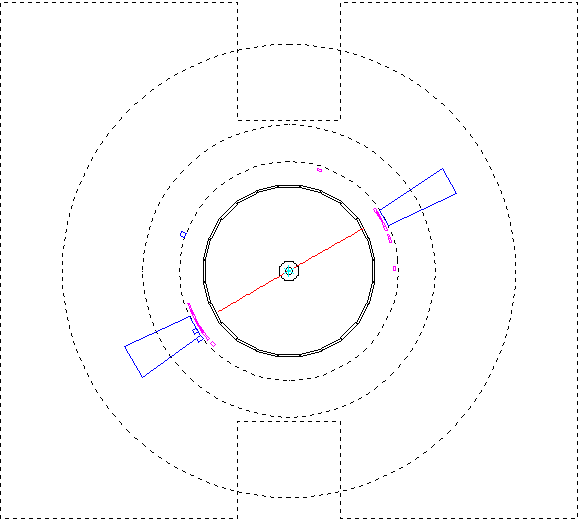
\includegraphics[width=0.8\linewidth]{figures/ee_02.png}
    \caption{Example for typical event of a decay into electrons. The characteristic feature of the decay into electrons is
    the very little number of trajectories and most of the energy submitted to first calorimeter (in the inner circle).}
\label{fig:ee}
\end{figure}

\begin{figure}[htpb]
    \centering
    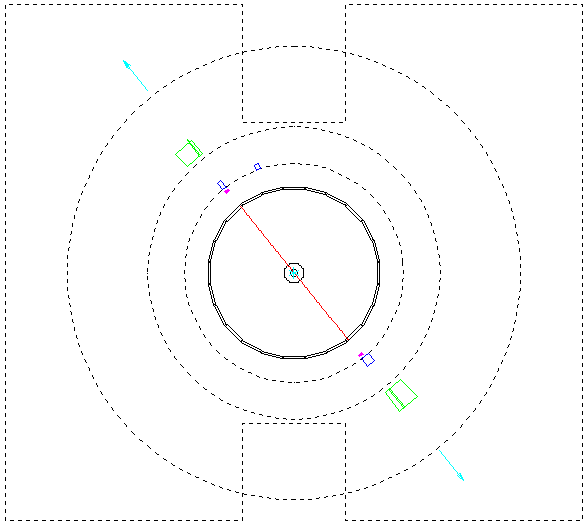
\includegraphics[width=0.8\linewidth]{figures/mm_02.png}
    \caption{Example for typical event of a decay into muons. As muons cannot be bound by the detector most of the time,
        a little amount of energy is absorbed by the first calorimeter. The muon detector far outside of this pictures (which
    is indicated by the turquoise arrows). }
\label{fig:mm}
\end{figure}

\begin{figure}[htpb]
    \centering
    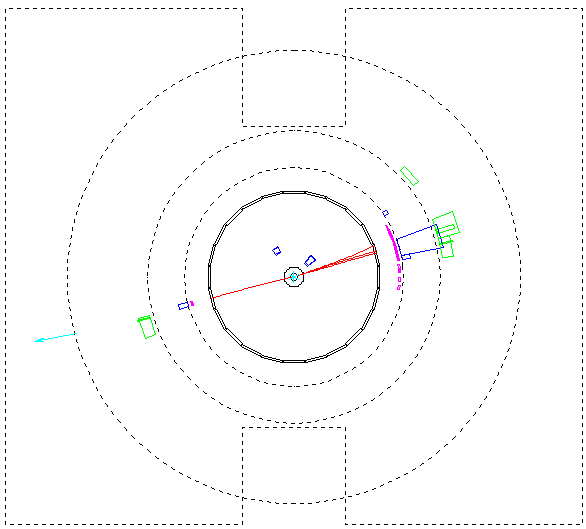
\includegraphics[width=0.8\linewidth]{figures/tt_02.png}
    \caption{Example for typical event of a decay into tauons. As the particles are not stopped in the first calorimeter,
    the probability of being electrons decreases significantly (this is not totally true as we will see later). Furthermore,
there is one particle escaping to the muon detector, but not two in opposite directions, as we would expect for muons. There
are also no hadron showers as characteristic for the quark branch. Hence we conclude this to be a taon event. }
\label{fig:tt}
\end{figure}

\begin{figure}[htpb]
    \centering
    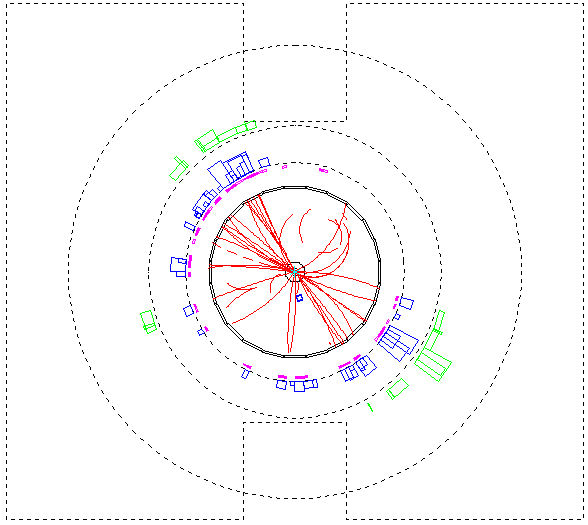
\includegraphics[width=0.8\linewidth]{figures/qq_02.png}
    \caption{Example for typical event of a decay into hadrons. As indicated in figure~\ref{fig:tt} hadronic shower are 
        a signature for quarks, originating from the \textbf{strong confinement}. 
        As bound states of quarks can only be found at low enough
   momentum, we observe a large creation of hadronic particles being measured in both of the calorimeter. More than half of
   the energy carried by incident hadrons is passed to additional secondaries. }
\label{fig:qq}
\end{figure}
\clearpage
\newpage
\subsection{Quantitative treatment}


